\def\referencePrismTikz
{
\begin{tikzpicture}
\label{reference_prism}
	\draw (0, 0, 0) -- (0, 0, 3.4);	
	\draw (0, 0, 0) -- (3.2, 0, 0);
	\draw (0, 0, 0) -- (0, 3.2, 0);
	\draw (0, 0, 2) -- (2, 0, 0);
	\draw (0, 2, 2) -- (2, 2, 0);
	\draw (2, 0, 0) -- (2, 2, 0);
	\draw (0, 0, 2) -- (0, 2, 2);
	\draw (0, 2, 2) -- (0,2,0);
	\draw (0, 2, 0) -- (2,2,0);
\end{tikzpicture}
}

\def\referencePyramidTikz
{
\begin{tikzpicture}[scale=2]
\label{reference_pyramid}
	\coordinate (o) at (0,0,0);
	\coordinate (e1) at (0,0,1);
	\coordinate (e2) at (1,0,0);
	\coordinate (e3) at (0,1,0);

	\draw (o) -- (e1) -- ($(e1)+(e2)$) -- (e2) -- (e3) -- 
			(o)-- (e2);
	\draw (e3) -- (e1);
	\draw (e3) -- ($(e1)+(e2)$);

\end{tikzpicture}
}

\def\macroTetraRegularity{  
\begin{figure}[!h]
  \centering
  \subfloat
  {
    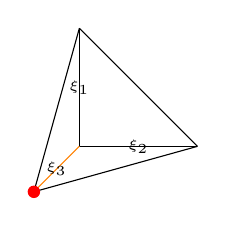
\begin{tikzpicture}[scale=1.5]
    \label{macro_tetra_reg}
      \draw (0.0,0.0,0.0) -- node[midway] {\tiny{\color{black}$\xi_1$}} (0.0,1.0,0.0);
      \draw (0.0,0.0,0.0) -- node[midway] {\tiny{\color{black}$\xi_2$}} (1.0,0.0,0.0);
      \draw (0.0,1.0,0.0) -- (1.0,0.0,0.0);
      \draw[orange] (0.0,0.0,0.0) -- node[midway] {\tiny{\color{black}$\xi_3$}} (0.0,0.0,1.0);
      \draw (0.0,1.0,0.0) -- (0.0,0.0,1.0);
      \draw (1.0,0.0,0.0) -- (0.0,0.0,1.0);
      \fill[red] (0,0,1) circle (1.5pt);
    \end{tikzpicture}
  }
  \caption{Tetrahedral Macroelement.}
\end{figure}
}

\def\macroPrismRegularity{  
\begin{figure}[!h]
  \centering
  \subfloat
  {
    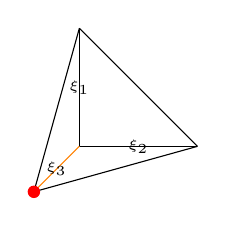
\begin{tikzpicture}[scale=1.5]
    \label{macro_prism_reg}
      \draw (0.0,0.0,0.0) -- node[midway] {\tiny{\color{black}$\xi_1$}} (0.0,1.0,0.0);
      \draw (0.0,0.0,0.0) -- node[midway] {\tiny{\color{black}$\xi_2$}} (1.0,0.0,0.0);
      \draw (0.0,1.0,0.0) -- (1.0,0.0,0.0);
      \draw[orange] (0.0,0.0,0.0) -- node[midway] {\tiny{\color{black}$\xi_3$}} (0.0,0.0,1.0);
      \draw (0.0,1.0,0.0) -- (0.0,0.0,1.0);
      \draw (1.0,0.0,0.0) -- (0.0,0.0,1.0);
      \fill[red] (0,0,1) circle (1.5pt);
    \end{tikzpicture}
  }
  \caption{Prismatic Macroelement.}
\end{figure}
}

\def\unitTangentsPyramid
{
\begin{tikzpicture}[scale=2,post/.style={->, shorten >=1pt, >=stealth', semithick}]
\label{reference_pyramid}
  \coordinate (o) at (0,0,0);
  \coordinate (e1) at (0,0,1);
  \coordinate (e2) at (1,0,0);
  \coordinate (e3) at (0,1,0);
  \coordinate (e4) at ($(e1)+(e2)$);

  \coordinate (a1start) at ($.2*(e1)$);
  \coordinate (a1end)   at ($.5*(e1)$);
  \coordinate (a2start)   at ($.8*(e1)+.2*(e4)$);
  \coordinate (a2end)   at ($.5*(e1)+.5*(e4)$);
  \coordinate (a3start)   at ($.8*(e2)+.2*(e4)$);
  \coordinate (a3end)   at ($.5*(e2)+.5*(e4)$);
  \coordinate (a4start) at ($.17*(e2)$);
  \coordinate (a4end)   at ($.4*(e2)$);
  \coordinate (a5start) at ($.2*(e3)$);
  \coordinate (a5end)   at ($.5*(e3)$);
  \coordinate (a6start) at ($.2*(e3)+.8*(e1)$);
  \coordinate (a6end)   at ($.5*(e3)+.5*(e1)$);
  \coordinate (a7start) at ($.2*(e3)+.8*(e2)$);
  \coordinate (a7end)   at ($.5*(e3)+.5*(e2)$);
  \coordinate (a8start) at ($.2*(e3)+.8*(e4)$);
  \coordinate (a8end)   at ($.5*(e3)+.5*(e4)$);

  \draw (o) -- (e1) -- ($(e1)+(e2)$) -- (e2) -- (e3) -- 
      (o)-- (e2);
  \draw (e3) -- (e1);
  \draw (e3) -- (e4);
  \foreach \i in {1,...,8}{
    \draw [post,very thick] (a\i start) -- (a\i end);
  }

\end{tikzpicture}
}

\def\unitTangentsPrism
{
\begin{tikzpicture}[scale=2,post/.style={->, shorten >=1pt, >=stealth', semithick}]
\label{reference_pyramid}
  \coordinate (o) at (0,0,0);
  \coordinate (e1) at (0,0,1);
  \coordinate (e2) at (1,0,0);
  \coordinate (e3) at (0,1,0);
  \coordinate (e4) at ($(e1)+(e3)$);
  \coordinate (e5) at ($(e2)+(e3)$);

  \coordinate (a1start) at ($.2*(e1)$);
  \coordinate (a1end)   at ($.5*(e1)$);
  \coordinate (a2start)   at ($.2*(e2)$);
  \coordinate (a2end)   at ($.5*(e2)$);

  \coordinate (a3start)   at ($.2*(e3)$);
  \coordinate (a3end)   at ($.5*(e3)$);

  \coordinate (a4start) at ($.83*(e3)+.17*(e4)$);
  \coordinate (a4end)   at ($.5*(e3)+.5*(e4)$);
  
  \coordinate (a5start) at ($.8*(e3)+.2*(e5)$);
  \coordinate (a5end)   at ($.5*(e3)+.5*(e5)$);
  
  \coordinate (a6start) at ($.2*(e4)+.8*(e1)$);
  \coordinate (a6end)   at ($.5*(e4)+.5*(e1)$);
  \coordinate (a7start) at ($.2*(e5)+.8*(e2)$);
  \coordinate (a7end)   at ($.5*(e5)+.5*(e2)$);
  \coordinate (a8start) at ($.2*(e4)+.8*(e5)$);
  \coordinate (a8end)   at ($.5*(e4)+.5*(e5)$);
  \coordinate (a9start) at ($.2*(e1)+.8*(e2)$);
  \coordinate (a9end)   at ($.5*(e1)+.5*(e2)$);

  \draw (o) -- (e1) -- (e2) -- (o) -- (e3) -- (e4) -- (e5) -- (e3);
  \draw (e4) -- (e1);
  \draw (e5) -- (e2);

  \foreach \i in {1,...,9}{
    \draw [post, very thick] (a\i start) -- (a\i end);
  }
\end{tikzpicture}
}